\documentclass[12pt]{article}

\usepackage[T1]{fontenc}
\usepackage{palatino}
\usepackage{amsmath,amssymb,amsthm}
\usepackage{geometry}
\usepackage{setspace}
\usepackage{hyperref}
\usepackage{tikz}
\usetikzlibrary{positioning,arrows.meta}
\usepackage{float}

\geometry{margin=1.25in}
\onehalfspacing

\newtheorem{theorem}{Theorem}
\newtheorem{proposition}[theorem]{Proposition}
\newtheorem{definition}[theorem]{Definition}
\newtheorem{remark}[theorem]{Remark}

\title{Rotation Before Number:\\
Admissibility, Geometry, and the Quotient Structure of Quantum Mechanics}
\author{Flyxion\\
\small Independent Researcher}
\date{June 2026}

\begin{document}

\maketitle

\begin{abstract}
A recent paper by Barrios Hita, Trushechkin, Kampermann, Epping, and Bru{\ss} establishes that quantum mechanics can be formulated entirely over the real numbers while reproducing all predictions of the complex theory \cite{Barrios}. This essay argues that the construction is a deep instance of a principle running through geometry, epistemology, and the theory of admissibility. The argument proceeds in three stages. First, drawing on Tristan Needham's geometric reinterpretation of complex analysis \cite{Needham}, we recover the claim that complex numbers are compact encodings of planar rotations, and that the real formulation is not an elimination but an \emph{explanatory recovery} of the generative mechanism those encodings compressed. Second, we connect this to the admissibility program: the quotient space that the paper constructs to handle composite systems is precisely an admissibility quotient, collapsing distinctions that are representationally present but physically unreachable. Third, we identify the novel contribution as establishing a three-level hierarchy---coordinates, representations, invariant structure---in which physical ontology belongs to the deepest layer alone. Ambiguity is conserved throughout, migrating from state vectors into gauge orbits. Complex numbers are not necessary to describe quantum mechanics; but the geometry they were encoding was always there, and the quotient reveals which distinctions belong to reality and which belong only to description.
\end{abstract}

%------------------------------------------------------------------
\section{Explanation Before Correctness}
%------------------------------------------------------------------

There is a distinction that Tristan Needham's \emph{Visual Complex Analysis} draws implicitly throughout its preface and opening chapters, though he never states it quite in these terms \cite{Needham}. It is the distinction between a representation that is \emph{correct} and one that is \emph{explanatory}.

A correct representation encodes the right answers. An explanatory representation makes the generative mechanism visible. The two need not coincide. A formalism can remain correct long after the geometric intuition that produced it has been compressed into notation and forgotten. When that compression happens, the notation continues to yield valid results while becoming epistemically opaque---capable of producing answers without revealing why those answers are true.

Needham's argument is not primarily that geometry is a helpful visualization of complex algebra. It is that the geometric interpretation is the \emph{source}: the algebra of complex numbers emerged historically from geometric reasoning about rotations and scalings in the plane, and the algebra compressed that geometry into notation. Visual reasoning is not a pedagogical aid appended to an algebraically prior subject. It is where the subject came from.

This gives us a distinction that will carry weight throughout the essay:
\[
\text{correct representation}
\;\neq\;
\text{explanatory representation.}
\]
The standard algebraic presentation of complex numbers is correct. Needham's geometric presentation is explanatory. The real-number formulation of quantum mechanics discussed below falls on the same axis: complex amplitudes remain correct, but the flag construction makes the underlying rotational mechanism visible again.

This is also the sense in which the title is meant. Rotation is not prior to number in the order of correctness---both the complex and the real descriptions yield the same predictions. Rotation is prior in the order of explanation. The number recorded the rotation. The rotation generated the number.

Because the essay draws repeatedly on the notion of admissibility, a working definition is useful before the term bears argumentative weight.

\begin{definition}[Admissibility]
An \emph{admissibility condition} is a rule that determines which distinctions correspond to physically realizable or operationally accessible differences and which are merely representational artifacts. An \emph{admissibility quotient} identifies and collapses all distinctions that fail this criterion, leaving the space of equivalence classes under the relation of operational indistinguishability.
\end{definition}

On this account, the passage from a raw representation to its admissibility quotient is a form of repair: not the correction of an error, but the removal of distinctions that were never genuine to begin with. The real formulation of quantum mechanics will provide a concrete mathematical instance of exactly this operation.

%------------------------------------------------------------------
\section{Rotation Before Number}
%------------------------------------------------------------------

With that distinction in hand, we can state Needham's geometric inversion precisely.

The standard story about complex numbers begins with the observation that $x^2 = -1$ has no real solution, introduces $i$ as a formal square root of $-1$, and ends with $\mathbb{C}$ as an extension field of $\mathbb{R}$ \cite{Gauss,Argand,Wessel}. In this story, complex numbers are algebraic objects first: points, scalars, coordinates satisfying field axioms. Their geometric interpretation is secondary.

Needham's inversion says: the algebra did not come first. What came first was the recognition that the plane admits a coherent family of combined rotations and scalings, and that these operations compose in a systematic way. The algebraic field structure is a compression: it records which compositions are admissible and how they combine, without explaining why those combinations are the natural ones. Figure~\ref{fig:needham-inversion} summarizes this inversion.

\begin{figure}[ht]
\centering
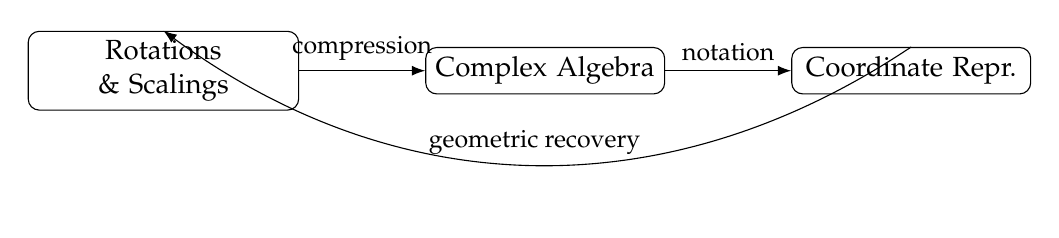
\begin{tikzpicture}[>=Latex, node distance=0.3cm and 1.6cm]
  \node (rot) [draw, rounded corners, text width=3.2cm, align=center]
    {Rotations \& Scalings};
  \node (alg) [draw, rounded corners, text width=2.8cm, align=center,
               right=of rot]
    {Complex Algebra};
  \node (coord) [draw, rounded corners, text width=2.8cm, align=center,
                 right=of alg]
    {Coordinate Repr.};

  \draw[->] (rot) -- node[above,font=\small]{compression} (alg);
  \draw[->] (alg) -- node[above,font=\small]{notation} (coord);
  \draw[->,bend left=35]
    (coord.north) to node[above,font=\small]{geometric recovery} (rot.north);
\end{tikzpicture}
\caption{Needham's inversion. Geometry generates algebra; algebra generates
notation. Explanatory recovery reconstructs the geometric structure hidden by
the notation.}
\label{fig:needham-inversion}
\end{figure}

On the geometric account, a complex number $z = re^{i\theta}$ is an \emph{operation}: the amplitwist that scales a vector by $r$ and rotates it by $\theta$. Needham introduces the word ``amplitwist'' precisely because no existing term captured the unity of the operation---existing vocabulary split a single stable phenomenon into two separate components, and the new word introduced a new admissible distinction.

Every nonzero complex number admits such a decomposition.

\begin{proposition}[Amplitude--Twist Decomposition]
Every nonzero complex number $z \in \mathbb{C}$ admits a unique decomposition
\[
z = r e^{i\theta}
\]
with $r > 0$ and $\theta \in [0, 2\pi)$.
\end{proposition}

\begin{proof}
For $z = x + iy$ with $(x,y) \neq (0,0)$, set $r = \sqrt{x^2 + y^2} > 0$.
Then $x/r = \cos\theta$ and $y/r = \sin\theta$ for a unique $\theta \in [0,2\pi)$.
Hence $z = r(\cos\theta + i\sin\theta) = re^{i\theta}$ by Euler's formula,
and uniqueness follows from the uniqueness of polar coordinates.
\end{proof}

The amplitude $r$ and the twist $\theta$ are thus genuinely independent:
\[
z \;=\; \underbrace{r}_{\text{amplitude}} \cdot \underbrace{e^{i\theta}}_{\text{twist}}.
\]
The notation fuses them, but the geometry keeps them separate. Figure~\ref{fig:amplitwist} makes this visible.

\begin{figure}[ht]
\centering
\begin{tikzpicture}[scale=1.2]
  \draw[->] (-2.2,0) -- (2.2,0) node[right]{$\operatorname{Re}$};
  \draw[->] (0,-2.2) -- (0,2.2) node[above]{$\operatorname{Im}$};
  \draw[gray] (0,0) circle (1.7);
  \draw[thick,->] (0,0) -- ({1.7*cos(40)},{1.7*sin(40)})
    node[right]{$re^{i\theta}$};
  \draw (0.55,0) arc (0:40:0.55);
  \node at (0.82,0.22) {$\theta$};
  \node[gray] at ({0.5*1.7*cos(20)},{0.5*1.7*sin(20)+0.35}) {$r$};
\end{tikzpicture}
\caption{An amplitwist decomposes into a radial amplitude component $r$
and an angular twist component $\theta$. Notation fuses them; geometry
keeps them distinct.}
\label{fig:amplitwist}
\end{figure}

Complex multiplication is composition of amplitwists:
\[
r_1 e^{i\theta_1} \cdot r_2 e^{i\theta_2} = (r_1 r_2)\, e^{i(\theta_1 + \theta_2)}.
\]
Scaling factors multiply. Rotation angles add. The multiplication rule is not assumed but \emph{explained}: it follows from the geometry of how rotations and scalings compose. The algebra emerges from the geometry.

This constitutes what we may call the \emph{Needham Principle}:

\begin{quote}
\emph{Transformations are ontologically prior to the coordinates used to describe them.}
\end{quote}

The following proposition makes this principle precise.

\begin{proposition}[Coordinate Independence of Transformation]
\label{prop:coord-indep}
Let $T \colon X \to X$ be a transformation and let $\phi_1, \phi_2 \colon X \to \mathbb{R}^n$ be two admissible coordinate systems. Then
\[
\phi_2 \circ T \circ \phi_2^{-1}
=
(\phi_2 \circ \phi_1^{-1})\,
(\phi_1 \circ T \circ \phi_1^{-1})\,
(\phi_1 \circ \phi_2^{-1}).
\]
Changing coordinates alters only the representation of $T$, not the transformation itself.
\end{proposition}

\begin{proof}
The identity holds by composition:
$\phi_2 \circ T \circ \phi_2^{-1}
= (\phi_2 \circ \phi_1^{-1}) \circ (\phi_1 \circ T \circ \phi_1^{-1}) \circ (\phi_1 \circ \phi_2^{-1})$.
The transition maps $\phi_2 \circ \phi_1^{-1}$ and $\phi_1 \circ \phi_2^{-1}$ are coordinate changes (similarity transforms); they conjugate the representation of $T$ without altering $T$ itself.
\end{proof}

The point on the unit circle is generated by the motion $e^{i\theta}$ as $\theta$ varies. The number is generated by the transformation. The symbol records the process. This priority runs throughout \emph{Visual Complex Analysis}: Needham consistently introduces Euler's formula through the dynamics of rotation rather than through algebraic power series. The continuously evolving rotation is primary; the formula describes it.

The imaginary unit, on this account, is the quarter-turn operator $i(v) = R_{90^\circ}(v)$. The equation $i^2 = -1$ is not a mysterious algebraic fact but a transparent geometric statement:
\[
i^2(v) = R_{90^\circ}\bigl(R_{90^\circ}(v)\bigr) = R_{180^\circ}(v) = -v.
\]
From the admissibility perspective, $i^2 = -1$ is an \emph{admissibility constraint on planar transformations}: the composition of two admissible quarter-turns produces the unique admissible half-turn, and the algebra records which geometric continuations remain distinguishable under that constraint.

Needham also warns against confusing the coordinate pair $(x, y)$ with the geometric point it represents. A complex number is a single geometric object---an amplitwist---that admits multiple descriptions. The pair $(x, y)$ is a representative; the geometric operation is the invariant object described by many coordinate systems. That is the admissibility lesson stated in geometric language, and it is the lesson the quotient construction will make precise.

%------------------------------------------------------------------
\section{The Flag Space and the Reappearance of Rotation}
%------------------------------------------------------------------

Barrios Hita, Trushechkin, Kampermann, Epping, and Bru{\ss} take Needham's priority claim seriously at the level of quantum mechanics \cite{Barrios}. Earlier work had explored whether real quantum mechanics could reproduce all predictions of the complex theory \cite{Stueckelberg,Myrheim,McKague}, and the experimental literature had established that naive real quantum theories without the correct composite-system structure cannot \cite{Renou}. The central obstacle is a dimension mismatch: a state in $\mathbb{C}^2 \otimes \mathbb{C}^2$ carries $8$ real parameters, while the naive real tensor product $\mathbb{R}^4 \otimes \mathbb{R}^4$ carries $16$. Naive extension overcounts; the excess represents representational distinctions with no physical content.

The Barrios et al.\ construction begins with the single-system map
\[
\mathcal{S}\colon |\psi\rangle \;\mapsto\;
\operatorname{Re}(|\psi\rangle) \otimes |0\rangle_F
+ \operatorname{Im}(|\psi\rangle) \otimes |1\rangle_F
=: |\tilde{\psi}\rangle,
\]
where the two-dimensional ``flag'' system $F$ records the real and imaginary parts. A global phase $e^{i\alpha}$ on $|\psi\rangle$ translates to a rotation $R_F(\alpha)$ on the flag:
\[
\mathcal{S}(e^{i\alpha}|\psi\rangle) = R_F(\alpha)\,\mathcal{S}(|\psi\rangle).
\]
The $\mathrm{U}(1)$ ambiguity of complex quantum mechanics corresponds to an $\mathrm{SO}(2)$ ambiguity in the real formulation: a flag rotation leaving all observables unchanged.

The operators compatible with this structure take the form
\[
\mathcal{T}(\Pi) = \operatorname{Re}(\Pi) \otimes I_F + \operatorname{Im}(\Pi) \otimes J_F,
\]
where the flag matrices are
\[
I_F = \begin{pmatrix} 1 & 0 \\ 0 & 1 \end{pmatrix},
\qquad
J_F = \begin{pmatrix} 0 & -1 \\ 1 & 0 \end{pmatrix}.
\]

The following proposition shows that this is not a coincidence but a direct realization of the complex multiplication structure.

\begin{proposition}[Real Realization of Complex Multiplication]
\label{prop:real-complex}
The matrix $J_F$ satisfies $J_F^2 = -I_F$. Moreover, for any $a, b, c, d \in \mathbb{R}$,
\[
(aI_F + bJ_F)(cI_F + dJ_F) = (ac - bd)I_F + (ad + bc)J_F,
\]
which reproduces the complex multiplication rule $(a + ib)(c + id) = (ac-bd) + i(ad+bc)$.
\end{proposition}

\begin{proof}
Direct computation:
$J_F^2 = \bigl(\begin{smallmatrix}0&-1\\1&0\end{smallmatrix}\bigr)^2
= \bigl(\begin{smallmatrix}-1&0\\0&-1\end{smallmatrix}\bigr) = -I_F$.
Then $(aI_F+bJ_F)(cI_F+dJ_F) = acI_F + adJ_F + bcJ_F + bdJ_F^2
= (ac-bd)I_F + (ad+bc)J_F$,
which matches the complex rule.
\end{proof}

The entire complex algebra has reappeared as real matrix operations. $J_F$ is the quarter-turn operator realized as an explicit $2\times2$ real matrix. The rotation that $i$ was always encoding has been made geometrically manifest. Figure~\ref{fig:real-complex} summarizes this chain.

\begin{figure}[ht]
\centering
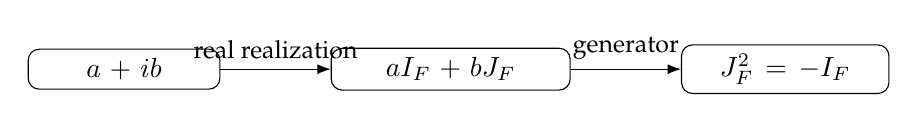
\begin{tikzpicture}[>=Latex, node distance=0.3cm and 1.4cm]
  \node (c) [draw, rounded corners, text width=2.2cm, align=center]
    {$a + ib$};
  \node (j) [draw, rounded corners, text width=2.8cm, align=center,
             right=of c]
    {$aI_F + bJ_F$};
  \node (r) [draw, rounded corners, text width=2.4cm, align=center,
             right=of j]
    {$J_F^2 = -I_F$};
  \draw[->] (c) -- node[above,font=\small]{real realization} (j);
  \draw[->] (j) -- node[above,font=\small]{generator} (r);
\end{tikzpicture}
\caption{Complex multiplication is realized in real vector spaces through
the distinguished rotation operator $J_F$ satisfying $J_F^2 = -I_F$. The
complex field becomes a derived structure.}
\label{fig:real-complex}
\end{figure}

The maps $\mathcal{S}$ and $\mathcal{T}$ satisfy
\[
\mathcal{S}(|\psi\rangle)^T \mathcal{T}(A)\, \mathcal{S}(|\psi\rangle) = \langle\psi|A|\psi\rangle
\]
for all states and operators \cite{Barrios}: all expectation values are preserved. The passage from complex to real formulation with flag structure is an explanatory recovery of the rotational geometry that complex notation compressed. A complex Hilbert space of dimension $n$ over $\mathbb{C}$ is equivalent, as a real structure, to a real Hilbert space of dimension $2n$ over $\mathbb{R}$ equipped with a distinguished operator $J$ satisfying $J^2 = -I$ \cite{Hall,Dyson,Arnold}. The complex numbers become secondary. The operator $J$---the rotation structure---is primary.

%------------------------------------------------------------------
\section{The Quotient as Admissibility}
%------------------------------------------------------------------

The single-system construction is straightforward. The real difficulty appears when one attempts to compose systems, and it is here that the admissibility program makes contact with the paper's central technical contribution.

The authors' postulate (P4) replaces the tensor product postulate with a physical locality requirement: given two subsystems, an operation on one must have no measurable effect on the other. Formally, any two local operators $O_A$ and $O_B$ must commute: $[O_A, O_B] = 0$ \cite{Barrios}. This postulate is satisfied automatically by the complex tensor product but is weaker than the tensor product postulate, allowing a different construction.

The naive extension $\mathcal{S}^{\otimes 2}$ is not well-defined: the states $|01\rangle_{AB} \otimes |00\rangle_{F_aF_b}$ and $-|01\rangle_{AB} \otimes |11\rangle_{F_aF_b}$ correspond to the same physical state yet are different vectors in the raw real tensor product. The kernel of $(\mathcal{S}^{-1})^{\otimes 2}$ is nontrivial, spanned by vectors of the form
\[
|\psi'\rangle_{AB} \otimes \bigl(|00\rangle_{F_aF_b} + |11\rangle_{F_aF_b}\bigr)
\quad\text{and}\quad
|\psi'\rangle_{AB} \otimes \bigl(|01\rangle_{F_aF_b} - |10\rangle_{F_aF_b}\bigr).
\]
The authors pass to the quotient space $\mathbb{R}^4_A \otimes \mathbb{R}^4_B / \ker[(\mathcal{S}^{-1})^{\otimes 2}]$. The canonical flag representatives of the two equivalence classes are
\[
|\psi^{(2)}_\text{even}\rangle = \tfrac{1}{\sqrt{2}}\bigl(|00\rangle_{F_aF_b} - |11\rangle_{F_aF_b}\bigr),
\qquad
|\psi^{(2)}_\text{odd}\rangle = \tfrac{1}{\sqrt{2}}\bigl(|01\rangle_{F_aF_b} + |10\rangle_{F_aF_b}\bigr).
\]
These are canonical representatives, not entangled states; each is equivalent to a product state. The quotient structure does the work that complex phase structure does automatically in $\mathbb{C}$.

Define an equivalence relation $\sim_A$ on the raw real state space $X$ by:
\[
x \sim_A x'
\quad \iff \quad
x \text{ and } x' \text{ are operationally indistinguishable by any admissible local measurement.}
\]

Before applying this relation, we verify it is an equivalence relation.

\begin{proposition}[Admissibility Equivalence]
\label{prop:equiv-rel}
The relation $\sim_A$ is an equivalence relation on $X$.
\end{proposition}

\begin{proof}
\emph{Reflexivity.} Every state is operationally indistinguishable from itself, since any measurement on $x$ returns the same statistics as on $x$.

\emph{Symmetry.} If no admissible measurement distinguishes $x$ from $x'$, then equally no admissible measurement distinguishes $x'$ from $x$.

\emph{Transitivity.} Suppose $x \sim_A y$ and $y \sim_A z$. Then for any admissible measurement $M$, the statistics of $M$ agree on $x$ and $y$, and on $y$ and $z$. Hence they agree on $x$ and $z$, so $x \sim_A z$.
\end{proof}

The quotient $X/{\sim_A}$ is therefore well-defined. The repair schema is:
\[
\text{Raw real tensor product}
\;\longrightarrow\;
\text{Distinction excess}
\;\longrightarrow\;
\text{Equivalence identification}
\;\longrightarrow\;
\text{Repaired composite space.}
\]
The repaired object is the equivalence class, not the representative. The construction is unique up to Hilbert space isomorphisms, given natural conditions related to $\mathrm{SO}(2)$ representations \cite{Barrios}. Figure~\ref{fig:quotient} illustrates the quotient map.

\begin{figure}[ht]
\centering
\begin{tikzpicture}[>=Latex]
  \draw (0,0) ellipse (2.2 and 1.4);
  \fill (0.8,0.6) circle (1.8pt);
  \fill (-0.7,-0.4) circle (1.8pt);
  \fill (0.2,-0.9) circle (1.8pt);
  \node[font=\small] at (1.0,0.85) {$x$};
  \node[font=\small] at (-0.9,-0.55) {$x'$};
  \node[font=\small] at (0.35,-1.1) {$x''$};
  \node at (0,-2.0) {$X$};
  \draw[->,thick] (3.0,0) -- (5.5,0) node[midway,above,font=\small]{$\pi$};
  \draw (7.5,0) circle (1.3);
  \node at (7.5,0) {$[x]$};
  \node at (7.5,-2.0) {$X/{\sim_A}$};
\end{tikzpicture}
\caption{The admissibility quotient $\pi\colon X \to X/{\sim_A}$ identifies
operationally indistinguishable states. Individual representatives are replaced
by equivalence classes.}
\label{fig:quotient}
\end{figure}

%------------------------------------------------------------------
\section{The Conservation of Ambiguity}
%------------------------------------------------------------------

A common expectation is that explanatory progress eliminates ambiguity. The real formulation shows something subtler. When the quotient construction repairs the state space, the ambiguity distributed across phase choices in the raw representation is not destroyed. It is reorganized---relocated from apparent freedom in state vectors into explicit structure in the equivalence relation. The lesson is not elimination but conservation: ambiguity redistributes rather than vanishes.

One of the more precise instances of this concerns global phase. In quantum mechanics, a global phase factor $e^{i\phi}$ has no observable consequences: $|\psi\rangle$ and $e^{i\phi}|\psi\rangle$ are physically identical \cite{Dirac,VonNeumann}. In the real formulation, this phase corresponds to a flag rotation $R_F(\phi)$ commuting with all physical operators.

The more subtle point concerns how phase distributes across composite systems. Given two independent subsystems, a global phase on the composite state can be split arbitrarily between the subsystems---what the paper calls ``phase kickback'' in the compositional setting \cite{Barrios}. In the real formulation, a global phase $e^{i\alpha}$ can be arbitrarily redistributed among the local flag rotations $R_{F_a}$, $R_{F_b}$, and so on. The equivalence relation on the flag states implements exactly this ambiguity.

The physically correct identification is:
\[
\text{physical state} = \text{gauge orbit,}
\]
not $\text{physical state} = \text{representative vector}$. The following proposition formalizes this conservation.

\begin{proposition}[Ambiguity Conservation]
\label{prop:ambig}
Let $G$ be a gauge group acting on state space $X$, and let $\pi\colon X \to X/G$ be the quotient map. Then the quotient does not eliminate gauge freedom but reorganizes it into the orbit structure of $G$.
\end{proposition}

\begin{proof}
Each equivalence class $[x] = \{gx : g \in G\}$ contains all gauge-related representatives. Passing to $X/G$ removes the need to choose a representative but does not remove the orbit itself. The freedom to choose among elements of $[x]$ is precisely the gauge freedom; it survives as the group action that generated the quotient. The total informational content of the gauge structure is therefore conserved.
\end{proof}

The ambiguity does not vanish. It transforms as shown in Figure~\ref{fig:ambiguity}:
\[
\text{ambiguity in state vectors}
\;\longrightarrow\;
\text{gauge freedom}
\;\longrightarrow\;
\text{orbit structure,}
\]
rather than $\text{ambiguity} \rightarrow 0$. The second path would represent genuine information destruction. The first represents reorganization.

\begin{figure}[ht]
\centering
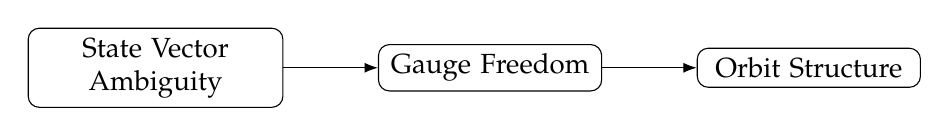
\begin{tikzpicture}[>=Latex, node distance=0.3cm and 1.2cm]
  \node (a) [draw, rounded corners, text width=3.0cm, align=center]
    {State Vector\\Ambiguity};
  \node (b) [draw, rounded corners, text width=2.6cm, align=center,
             right=of a]
    {Gauge Freedom};
  \node (c) [draw, rounded corners, text width=2.6cm, align=center,
             right=of b]
    {Orbit Structure};
  \draw[->] (a) -- (b);
  \draw[->] (b) -- (c);
\end{tikzpicture}
\caption{Ambiguity is not destroyed by quotienting. It is reorganized from
representational freedom in state vectors into gauge-orbit structure in the
quotient space.}
\label{fig:ambiguity}
\end{figure}

%------------------------------------------------------------------
\section{Witnesses and Invariant Structure}
%------------------------------------------------------------------

There is a natural connection between the quotient construction and the notion of a witness. A witness is not the underlying object. It is a structure that survives projection or representation change: what persists across admissible transformations.

In the quantum case, the complex phase of an individual state vector is not a witness. It does not survive the passage to physical predictions. The individual representative vector is therefore not the real object. The equivalence class is the real object, because it is the class that survives all admissible observations.

\begin{proposition}[Witness Invariance]
\label{prop:witness-inv}
Let $R_1$ and $R_2$ be admissible representations of a physical system related by an admissibility-preserving equivalence $R_1 \sim_A R_2$. Then any operational witness $W$ satisfies
\[
W(R_1) = W(R_2).
\]
Hence witnesses descend naturally to equivalence classes: the map $[R] \mapsto W(R)$ is well-defined on the quotient $X / {\sim_A}$.
\end{proposition}

\begin{proof}
Suppose $R_1 \sim_A R_2$. Then by definition no admissible measurement distinguishes $R_1$ from $R_2$. An operational witness $W$ is defined precisely as a quantity determined by admissible measurements. Therefore $W$ must return the same value on $R_1$ and $R_2$. The map $[R] \mapsto W(R)$ is thus well-defined on the equivalence class.
\end{proof}

The previous proposition leads directly to a sufficiency criterion.

\begin{proposition}[Witness Sufficiency]
\label{prop:witness-suff}
Suppose $x, y \in X$ satisfy $W(x) = W(y)$ for every admissible witness $W$. Then $x \sim_A y$.
\end{proposition}

\begin{proof}
Suppose for contradiction that $x \not\sim_A y$. Then some admissible measurement distinguishes $x$ from $y$, and that measurement defines an admissible witness $W$ with $W(x) \neq W(y)$, contradicting the assumption. Hence $x \sim_A y$.
\end{proof}

Together, Witness Invariance and Witness Sufficiency establish that the admissibility relation $\sim_A$ is \emph{exactly} the witness-indistinguishability relation: $x \sim_A y$ if and only if $W(x) = W(y)$ for all admissible witnesses $W$. Figure~\ref{fig:witnesses} illustrates how witnesses factor through the quotient.

\begin{figure}[ht]
\centering
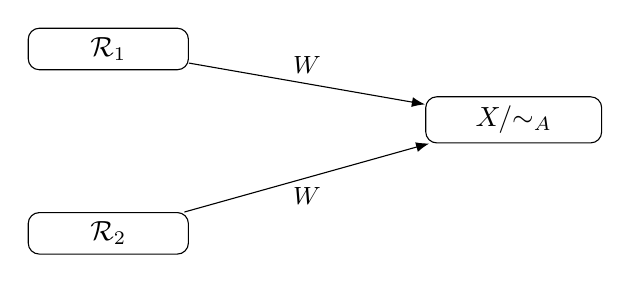
\begin{tikzpicture}[>=Latex, node distance=0.6cm and 2.5cm]
  \node (r1) [draw, rounded corners, text width=1.8cm, align=center]
    {$\mathcal{R}_1$};
  \node (r2) [draw, rounded corners, text width=1.8cm, align=center,
              below=1.8cm of r1]
    {$\mathcal{R}_2$};
  \node (q)  [draw, rounded corners, text width=2.0cm, align=center,
              right=3cm of r1, yshift=-0.9cm]
    {$X/{\sim_A}$};
  \draw[->] (r1) -- node[above,font=\small]{$W$} (q);
  \draw[->] (r2) -- node[below,font=\small]{$W$} (q);
\end{tikzpicture}
\caption{Distinct representations $\mathcal{R}_1$ and $\mathcal{R}_2$ induce
the same quotient of admissible distinctions. Operational witnesses $W$ factor
through the quotient and cannot distinguish between the representations.}
\label{fig:witnesses}
\end{figure}

In the quantum case, $W$ is any observable quantity: a transition probability, an expectation value, an interference pattern. These are functions of the gauge orbit. The expectation-value identity $\mathcal{S}(|\psi\rangle)^T \mathcal{T}(A)\,\mathcal{S}(|\psi\rangle) = \langle\psi|A|\psi\rangle$ \cite{Barrios} guarantees this at the formal level.

The slogan is: \emph{what persists across representations is what is real}. The rotation structure $J$ persists. The particular encoding of $J$---as multiplication by $i$ or as the flag matrix $J_F$---does not persist as a canonical object. The rotation is the witness. The coordinate representation of the rotation is the artifact.

%------------------------------------------------------------------
\section{Algebra Hides Geometry}
%------------------------------------------------------------------

The broader lesson generalizes. Algebra, when powerful, tends to compress the geometric information that generated it into symbolic operations. The geometric content becomes invisible inside the notation. Later generations inherit the algebra without the geometry. The notation becomes correct but epistemically opaque \cite{Penrose,Weyl}.

The history of complex numbers exemplifies this exactly. The original geometric content---rotation and scaling in the plane---was present from the beginning in the work of Wessel, Argand, and Gauss \cite{Wessel,Argand,Gauss}. But as complex analysis became a powerful computational tool, the geometric origin receded. By the time quantum mechanics was formulated, complex numbers were understood primarily as algebraic objects satisfying field axioms.

Needham's project is a recovery of the geometry from within the algebra \cite{Needham}. The flag-space paper is the same recovery applied to the quantum formalism. By making the rotation explicit as a real matrix $J_F$ rather than leaving it compressed inside the symbol $i$, the paper restores explanatory transparency: not repairing a mistake, but recovering the explanatory mechanism the formalism had compressed away while remaining correct.

The general pattern is:
\[
\text{geometry}
\;\longrightarrow\;
\text{algebra that encodes geometry}
\;\longrightarrow\;
\text{notation that hides encoding}
\;\longrightarrow\;
\text{correctness without explanation.}
\]
Recovery follows the same path in reverse:
\[
\text{correct but opaque}
\;\longrightarrow\;
\text{geometric reinterpretation}
\;\longrightarrow\;
\text{explanatory formulation.}
\]
When algebra hides geometry, the geometric distinctions are present in the formalism but not operationally accessible to someone working purely symbolically. The geometric reinterpretation makes those distinctions accessible again.

%------------------------------------------------------------------
\section{The Ontology of Quantum Mechanics}
%------------------------------------------------------------------

The philosophical conclusion is unusually strong. Complex numbers are not necessary to describe quantum mechanics. The Barrios et al.\ construction is a one-to-one mapping of complex quantum mechanics to a real description compatible with all quantum experiments, including multipartite Bell-type scenarios \cite{Barrios}. Physical reality depends only on the invariant structure preserved under the quotient.

To make this precise, separate three distinct layers:
\[
\text{Coordinates}
\;\longrightarrow\;
\text{Representations}
\;\longrightarrow\;
\text{Invariant Structure.}
\]
The field $\mathbb{C}$ and the pair $(\mathbb{R}^{2n}, J)$ both belong to the \emph{representation layer}: choices of how to coordinatize the state space. The quotient structure---the space of gauge orbits, the admissibility manifold---belongs to the \emph{invariant layer}: what all admissible representations share. The coordinates layer comprises further choices within a representation: basis, phase convention, gauge.

Physical ontology belongs to the invariant layer alone. The following proposition makes this explicit, connecting Witness Sufficiency to the ontological conclusion.

\begin{proposition}[Ontological Invariance]
\label{prop:ont-inv}
Let $\mathcal{R}_1$ and $\mathcal{R}_2$ be admissible representations of a physical theory. If there exists an isomorphism $\Phi\colon \mathcal{R}_1/{\sim_A} \to \mathcal{R}_2/{\sim_A}$ preserving all operational witnesses---that is, $W(\mathcal{R}_1) = W(\Phi(\mathcal{R}_2))$ for every witness $W$---then $\mathcal{R}_1$ and $\mathcal{R}_2$ possess identical ontological content. All differences between them are representational rather than physical.
\end{proposition}

\begin{proof}
By Witness Invariance (Proposition~\ref{prop:witness-inv}), every operational witness $W$ is well-defined on the quotient $X/{\sim_A}$. By Witness Sufficiency (Proposition~\ref{prop:witness-suff}), the admissibility relation is exactly witness-indistinguishability. If $\Phi$ preserves all witnesses, then no operational procedure can distinguish $\mathcal{R}_1$ from $\mathcal{R}_2$. Since the physical content of a theory is exhausted by what is operationally accessible, any remaining difference between $\mathcal{R}_1$ and $\mathcal{R}_2$ is necessarily representational.
\end{proof}

In the quantum case, $\mathcal{R}_1 = \mathbb{C}^n$ and $\mathcal{R}_2 = (\mathbb{R}^{2n}, J_F)$ satisfy the conditions of Ontological Invariance: the expectation-value identity guarantees the required witness-preserving isomorphism. The complex and real formulations are therefore not two theories but two coordinate systems on the same theory.

The novel contribution of this essay is not the claim that complex numbers are rotations. Needham established that perspective decades ago \cite{Needham}. The novel chain is:
\[
\text{Rotation}
\;\longrightarrow\;
\text{Equivalence}
\;\longrightarrow\;
\text{Admissibility.}
\]
Figure~\ref{fig:architecture} shows the logical architecture of the entire argument.

\begin{figure}[ht]
\centering
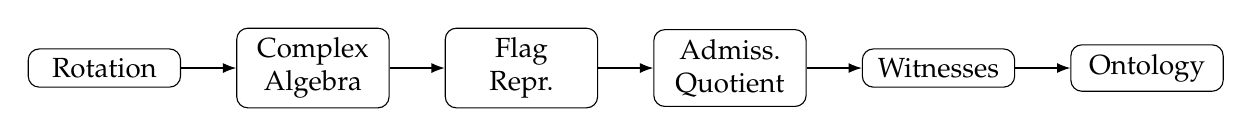
\begin{tikzpicture}[>=Latex, node distance=0.25cm and 0.7cm]
  \node (rot)  [draw, rounded corners, text width=1.7cm, align=center]
    {Rotation};
  \node (alg)  [draw, rounded corners, text width=1.7cm, align=center,
                right=of rot]
    {Complex\\Algebra};
  \node (flag) [draw, rounded corners, text width=1.7cm, align=center,
                right=of alg]
    {Flag\\Repr.};
  \node (quot) [draw, rounded corners, text width=1.7cm, align=center,
                right=of flag]
    {Admiss.\\Quotient};
  \node (wit)  [draw, rounded corners, text width=1.7cm, align=center,
                right=of quot]
    {Witnesses};
  \node (ont)  [draw, rounded corners, text width=1.7cm, align=center,
                right=of wit]
    {Ontology};
  \draw[->] (rot)--(alg);
  \draw[->] (alg)--(flag);
  \draw[->] (flag)--(quot);
  \draw[->] (quot)--(wit);
  \draw[->] (wit)--(ont);
\end{tikzpicture}
\caption{Logical architecture of the essay. The argument moves from geometric
rotation through algebraic encoding and the flag representation to the quotient
structure, witnesses, and finally ontological invariants.}
\label{fig:architecture}
\end{figure}

The essay begins as a discussion of complex numbers and ends as a discussion of which distinctions deserve ontological status. That transition is where the admissibility framework adds something genuinely new: a principled account of why the quotient is not merely a technical convenience but the location of physical reality.

Needham's deepest contribution to this essay is not the rotation interpretation of $i$. It is the practice of asking, at every step, what geometric operation survives when the notation changes. That is precisely the question the admissibility quotient answers at the level of quantum mechanics.

The rotational structure survives a change of coordinates, while the coordinates themselves do not. The geometry was always there; the quotient reveals which distinctions belong to reality and which belong only to description. The repaired object is therefore not the representative but the equivalence class itself. As Barrios et al.\ conclude: complex numbers are not necessary to describe quantum mechanics---but they are certainly very useful \cite{Barrios}.

%------------------------------------------------------------------
\begin{thebibliography}{99}

\bibitem{Needham}
T.\ Needham,
\textit{Visual Complex Analysis},
Oxford University Press, Oxford (1997).

\bibitem{Barrios}
P.\ Barrios Hita, A.\ Trushechkin, H.\ Kampermann, M.\ Epping,
and D.\ Bru{\ss},
``Quantum Mechanics Based on Real Numbers: A Consistent Description,''
\textit{Physical Review Letters} \textbf{136}, 240202 (2026).

\bibitem{Renou}
M.-O.\ Renou et al.,
``Quantum Theory Based on Real Numbers Can Be Experimentally Falsified,''
\textit{Nature} \textbf{600}, 625--629 (2021).

\bibitem{McKague}
M.\ McKague, M.\ Mosca, and N.\ Gisin,
``Simulating Quantum Systems Using Real Hilbert Spaces,''
\textit{Physical Review Letters} \textbf{102}, 020505 (2009).

\bibitem{Myrheim}
J.\ Myrheim,
``Quantum Mechanics on Real Hilbert Spaces,''
arXiv:quant-ph/9905037 (1999).

\bibitem{Stueckelberg}
E.\ C.\ G.\ Stueckelberg,
``Quantum Theory in Real Hilbert Space,''
\textit{Helvetica Physica Acta} \textbf{33}, 727--752 (1960).

\bibitem{Dyson}
F.\ J.\ Dyson,
``The Threefold Way: Algebraic Structure of Symmetry Groups and Ensembles
in Quantum Mechanics,''
\textit{Journal of Mathematical Physics} \textbf{3}, 1199--1215 (1962).

\bibitem{VonNeumann}
J.\ von Neumann,
\textit{Mathematical Foundations of Quantum Mechanics},
Princeton University Press, Princeton (1955).

\bibitem{Dirac}
P.\ A.\ M.\ Dirac,
\textit{The Principles of Quantum Mechanics}, 4th ed.,
Oxford University Press, Oxford (1958).

\bibitem{BirkhoffNeumann}
G.\ Birkhoff and J.\ von Neumann,
``The Logic of Quantum Mechanics,''
\textit{Annals of Mathematics} \textbf{37}, 823--843 (1936).

\bibitem{Jauch}
J.\ M.\ Jauch,
\textit{Foundations of Quantum Mechanics},
Addison-Wesley, Reading, MA (1968).

\bibitem{Varadarajan}
V.\ S.\ Varadarajan,
\textit{Geometry of Quantum Theory}, 2nd ed.,
Springer, New York (1985).

\bibitem{Hall}
B.\ C.\ Hall,
\textit{Quantum Theory for Mathematicians},
Springer, New York (2013).

\bibitem{Arnold}
V.\ I.\ Arnold,
\textit{Mathematical Methods of Classical Mechanics}, 2nd ed.,
Springer, New York (1989).

\bibitem{Weyl}
H.\ Weyl,
\textit{Symmetry},
Princeton University Press, Princeton (1952).

\bibitem{Penrose}
R.\ Penrose,
\textit{The Road to Reality},
Jonathan Cape, London (2004).

\bibitem{Gauss}
C.\ F.\ Gauss,
\textit{Theoria Residuorum Biquadraticorum},
Commentationes Societatis Regiae Scientiarum Gottingensis Recentiores
\textbf{6} (1831).

\bibitem{Argand}
J.-R.\ Argand,
\textit{Essai sur une mani\`{e}re de repr\'{e}senter les quantit\'{e}s
imaginaires dans les constructions g\'{e}om\'{e}triques},
Paris (1806).

\bibitem{Wessel}
C.\ Wessel,
``On the Analytical Representation of Direction,''
\textit{Danske Videnskabernes Selskabs Skrifter} \textbf{5} (1799).

\end{thebibliography}

\end{document}
